\documentclass[../main.tex]{subfiles}

\begin{document}


\subsection{Minería de textos}

El término minería tiene el significado de "búsqueda, descubrimiento, inducción y refinamiento". Por lo tanto, se trata de analizar textos y extraer conclusiones. El usuario espera respuestas y conclusiones a las preguntas de interés, en lugar de numerosos resultados de búsqueda, dejando que sea la máquina quien analice y encuentre respuestas. Está basada en diferentes tecnologías, originada de técnicas como clasificación de textos, agrupación de textos, y resumen automático de textos. Tiene aplicaciones en campos como la economía, servicios de información, gestión social, seguridad nacional.

Existen dos aspectos a tener en cuenta sobre el contenido del texto: no está estructurado y está descrito por el lenguaje natural, no por datos. 

La minería de textos se puede clasificar en:

\begin{itemize}
	\item Las preguntas son claras y específicas pero no se conoce respuesta.
	\item Se conoce el propósito general pero no se tienen preguntas definidas y específicas.
\end{itemize}

No consiste en un sistema único, si no la aplicación integrada de varias tecnologías, entra las que se pueden encontrar:

\begin{itemize}
	\item Clasificación de textos. Es una tecnología de clasificación de patrones: clasifica un texto de acuerdo a su contenido.
	\item Agrupación de textos. Divide el texto en diferentes categorías. Se diferencia del método anterior en que el número de categorías no está predeterminado.
	\item Modelo de temas. Son modelos estadísticos que extraen temas y conceptos que se esconden tras las palabras del texto.
	\item Análisis emocional del texto y minería de opiniones. Se basa en información subjetiva, como puntos de vista o actitudes, dentro de un rango negativo-positivo.
	\item Detección y seguimiento de tema. Extrae y muestra temas desde diferentes noticias y comentarios. Especialmente interesante son los temas candentes, de los que más «se habla».
	\item Extracción de información. Consiste en extraer información útil y estructurada desde textos sin estructura o semiestructurados. Información como reconocimiento de entidades, desambiguación de entidades, extracción de relaciones, extracción de eventos.
	\item Resumen automático de textos. Genera un resumen empleando métodos de procesamiento de lenguaje natural.
\end{itemize}

\textbf{Procesamiento de Lenguaje Natural}

El procesamiento de lenguaje natural (en inglés Natural Language Processing, NLP) forma parte de la minería de textos y por extensión de la inteligencia artificial. Consiste en la habilidad de comprender un texto hablado o escrito del mismo modo que lo haría un ser humano.


\subsection{Portable Document Format}

Portable Document Format o PDF es un formato de fichero que se emplea para representar documentos. Fue creado por Adobe Systems Incorporated en 1993. Su uso está bastante extendido por la facilidad que ofrece para visualizar e intercambiar documentos, independientemente del entorno en el que fueron creados o en el que serán visualizados.

Un documento PDF puede incluir metadatos. Estos se pueden almacenar de dos formas distintas: como un diccionario de información del documento (Document Information Dictionary) o como flujo de metadatos (Metadata Stream)

El diccionario de información del documento era forma original de inclusión de metadatos. A partir de la versión 1.4, se añadió el flujo de metadatos. De los dos métodos, que pueden convivir en el mismo fichero, el segundo es el preferido.


\subsection{Dublin Core}

Dublin Core es un estándar de representación de metadatos para la descripción de recursos. Consiste en un conjunto de quince elementos. Cada uno de ellos posee un nombre bastante descriptivo de modo que sea más comprensible su contenido.

\begin{figure}[h]
  \centering
  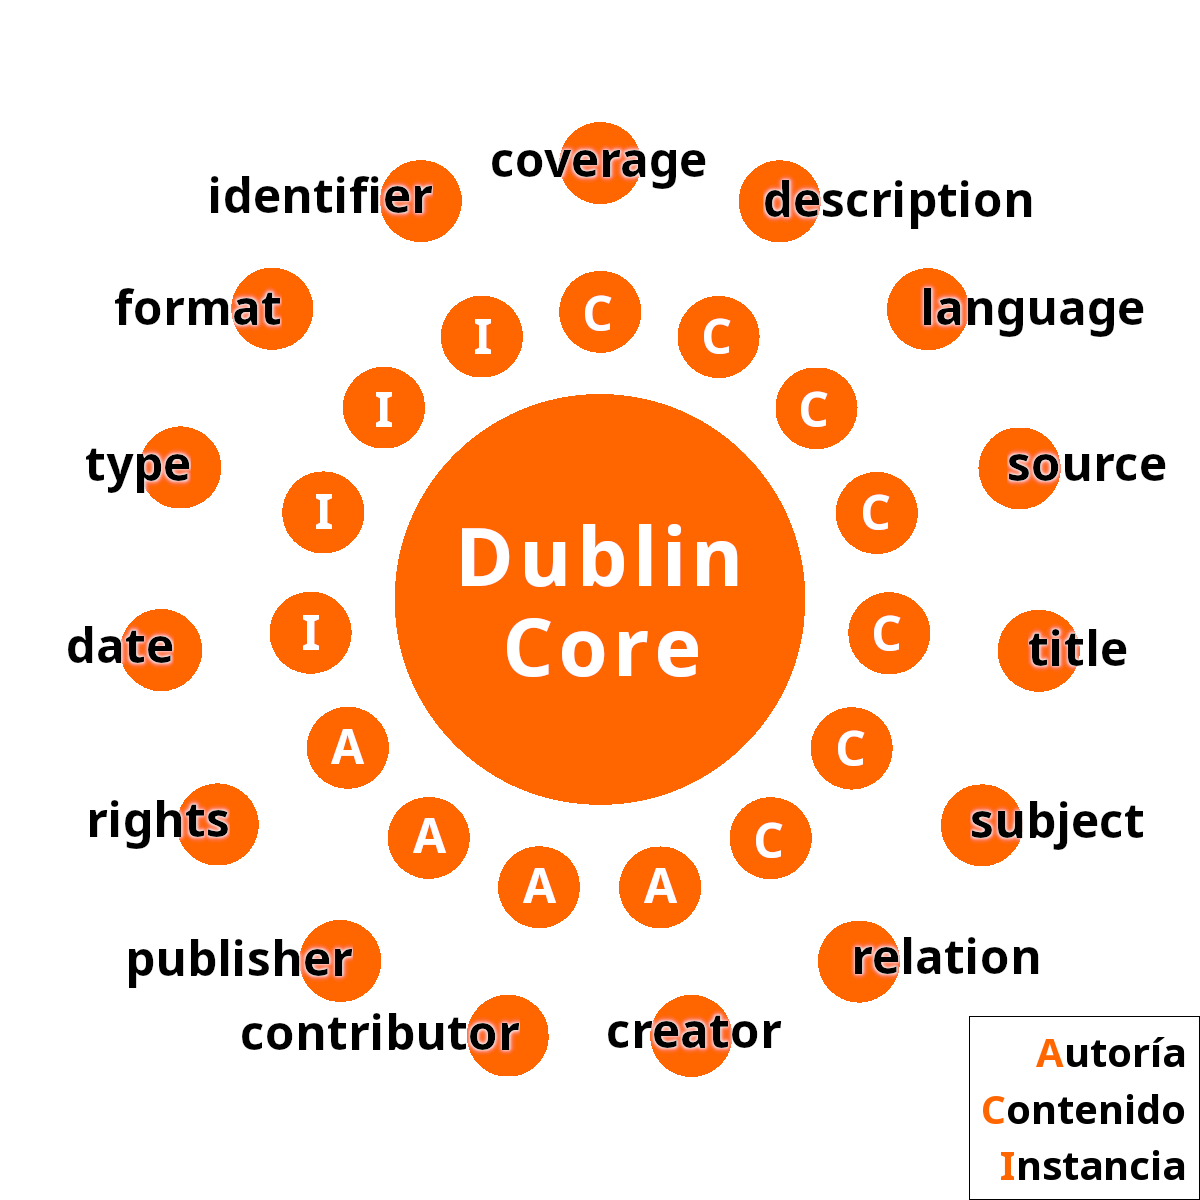
\includegraphics[width=0.7\textwidth]{../images/dublincore.png}
  \caption{Logo de Dublin Core con sus quince elementos.}
\end{figure}

Los quince elementos son los siguientes:

\begin{description}

  \item[contributor] \mbox{}\\ Es la persona u organización que ha hecho contribuciones intelectuales significativas al recurso. Su contribución es secundaria, no se especifica en la etiqueta \texttt{creator}. Se utiliza por ejemplo, en el caso de los libros, para el traductor o el editor.

  \item[coverage] \mbox{}\\ Son las características espaciales o temporales del contenido intelectual del recurso. La cobertura espacial se refiere a una región física (por ejemplo, un sector celeste) utilizando nombres de lugares o coordenadas (por ejemplo, longitud y latitud). La cobertura temporal se refiere al tema del recurso y no a la fecha de su creación o puesta a disposición (esta última pertenece al elemento fecha). La cobertura temporal se suele especificar utilizando períodos de tiempo con nombre (por ejemplo, el Neolítico) o el mismo formato de fecha/hora que se recomienda para el elemento.

  \item[creator] \mbox{}\\ Es la persona u organización responsable (principalmente) de la creación del contenido intelectual del recurso. Se utiliza por ejemplo, para los escritores que firman un libro.

  \item[date] \mbox{}\\ Es la fecha asociada a un evento del recurso. Normalmente la fecha de publicación o creación. Se recomienda utilizar la norma ISO 8601, que tiene el formato \texttt{AAAA} y \texttt{AAAA-MM-DD}, siendo \texttt{AAAA} el año, \texttt{MM} el mes y \texttt{DD} el día.

  \item[description] \mbox{}\\ Es la descripción textual del contenido del recurso. Suele ser un resumen del contenido en el caso de recursos escritos.

  \item[format] \mbox{}\\ Es el formato de los datos. Puede incluir información extra como las dimensiones o la duración. Tiene su utilidad para identificar las herramientas necesarias para poder visualizar el recurso.

  \item[identifier] \mbox{}\\ Es un texto o número utilizado para identificar de forma inequívoca el recurso. Por ejemplo, el ISBN en el caso de los libros o el DOI para los artículos científicos.

  \item[language] \mbox{}\\ Es el idioma del contenido intelectual del recurso. Se recomienda utilizar los códigos de idioma IETF, recogidos en la norma RFC 1766.

  \item[publisher] \mbox{}\\ Es la entidad responsable de que el recurso esté disponible en su forma actual, como una editorial o un departamento universitario.

  \item[relation] \mbox{}\\ Es un identificador de un recurso secundario y su relación con el recurso actual. Este elemento se usa para vincular recursos relacionados.

  \item[rights] \mbox{}\\ Es una declaración de gestión de derechos. Suele enlazar con información sobre los derechos de uso del recurso.

  \item[source] \mbox{}\\ Es la fuente de la que se deriva el recurso actual. Solo se utiliza cuando este recurso secundario se considere relevante para el descripción del recurso presente.

  \item[subject] \mbox{}\\ Es el asunto, tema o materia que define el recurso. Se suele expresar con palabras clave o frases descriptivas. Para facilitar la interoperatividad se utilizan vocabularios controlados o sistemas de clasificación formales.

  \item[title] \mbox{}\\ Es el título dado al recurso, normalmente por parte del autor o del editor.

  \item[type] \mbox{}\\ Es la categoría del recurso. Por ejemplo, una novela, un ensayo o informe técnico.

\end{description}


\end{document}
